\chapter{Other Elements}

This section shows you how to add other elements, like figurs or tables, to your document.

\section{Tables}

\subsection{Simple}

\begin{center}
\begin{tabular}{lrr}
	\toprule
	Description & Count & Price (single)\\
	\midrule
	Soda & 6 & 2.49 €\\
	Coffee & 2 & 3.19 €\\
	Sandwich & 1 & 5.39 €\\
	\bottomrule
\end{tabular}
\end{center}

\subsection{Specific Width}

\begin{center}
\begin{tabularx}{0.75\textwidth}{Xrr}
	\toprule
	Description & Count & Price (single)\\
	\midrule
	Soda & 6 & 2.49 €\\
	Coffee & 2 & 3.19 €\\
	Sandwich & 1 & 5.39 €\\
	\bottomrule
\end{tabularx}
\end{center}

\subsection{With Caption}

\Cref{tbl:some_table} as a caption and can be referenced.
Note that by using the \texttt{table} environment, the table is no longer inline and is repositioned automatically.

\begin{table}
	\centering
	\begin{tabularx}{0.75\textwidth}{Xrr}
		\toprule
		Description & Count & Price (single)\\
		\midrule
		Soda & 6 & 2.49 €\\
		Coffee & 2 & 3.19 €\\
		Sandwich & 1 & 5.39 €\\
		\bottomrule
	\end{tabularx}
	\caption{This table has a caption.}
	\label{tbl:some_table}
\end{table}

\section{Graphics}

Avoid having inline figures.
Always give them a caption and reference them in text.

\subsection{Figures}

See \cref{fig:some_figure}.

\begin{figure}
	\centering
	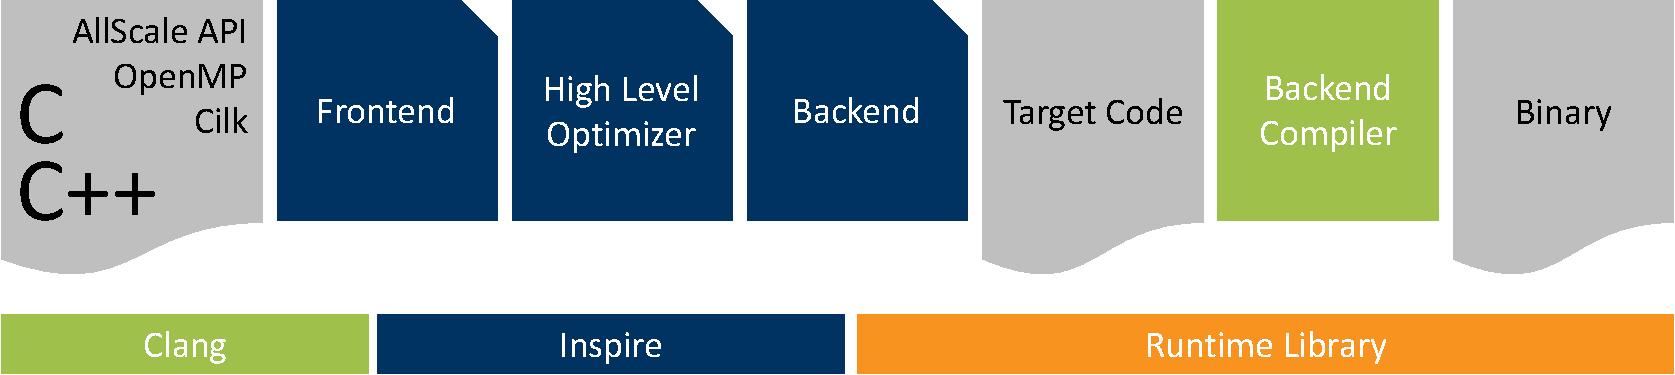
\includegraphics[width=0.9\textwidth]{images/example.pdf}
	\caption{An example image.}
	\label{fig:some_figure}
\end{figure}

\subsection{Plots}

See \cref{fig:some_plot}.

\begin{figure}
	\centering
	%% Creator: Matplotlib, PGF backend
%%
%% To include the figure in your LaTeX document, write
%%   \input{<filename>.pgf}
%%
%% Make sure the required packages are loaded in your preamble
%%   \usepackage{pgf}
%%
%% Figures using additional raster images can only be included by \input if
%% they are in the same directory as the main LaTeX file. For loading figures
%% from other directories you can use the `import` package
%%   \usepackage{import}
%% and then include the figures with
%%   \import{<path to file>}{<filename>.pgf}
%%
%% Matplotlib used the following preamble
%%
\begingroup%
\makeatletter%
\begin{pgfpicture}%
\pgfpathrectangle{\pgfpointorigin}{\pgfqpoint{4.000000in}{3.500000in}}%
\pgfusepath{use as bounding box, clip}%
\begin{pgfscope}%
\pgfsetbuttcap%
\pgfsetmiterjoin%
\definecolor{currentfill}{rgb}{1.000000,1.000000,1.000000}%
\pgfsetfillcolor{currentfill}%
\pgfsetlinewidth{0.000000pt}%
\definecolor{currentstroke}{rgb}{1.000000,1.000000,1.000000}%
\pgfsetstrokecolor{currentstroke}%
\pgfsetdash{}{0pt}%
\pgfpathmoveto{\pgfqpoint{0.000000in}{0.000000in}}%
\pgfpathlineto{\pgfqpoint{4.000000in}{0.000000in}}%
\pgfpathlineto{\pgfqpoint{4.000000in}{3.500000in}}%
\pgfpathlineto{\pgfqpoint{0.000000in}{3.500000in}}%
\pgfpathclose%
\pgfusepath{fill}%
\end{pgfscope}%
\begin{pgfscope}%
\pgfsetbuttcap%
\pgfsetmiterjoin%
\definecolor{currentfill}{rgb}{1.000000,1.000000,1.000000}%
\pgfsetfillcolor{currentfill}%
\pgfsetlinewidth{0.000000pt}%
\definecolor{currentstroke}{rgb}{0.000000,0.000000,0.000000}%
\pgfsetstrokecolor{currentstroke}%
\pgfsetstrokeopacity{0.000000}%
\pgfsetdash{}{0pt}%
\pgfpathmoveto{\pgfqpoint{0.500000in}{0.385000in}}%
\pgfpathlineto{\pgfqpoint{3.600000in}{0.385000in}}%
\pgfpathlineto{\pgfqpoint{3.600000in}{3.080000in}}%
\pgfpathlineto{\pgfqpoint{0.500000in}{3.080000in}}%
\pgfpathclose%
\pgfusepath{fill}%
\end{pgfscope}%
\begin{pgfscope}%
\pgfpathrectangle{\pgfqpoint{0.500000in}{0.385000in}}{\pgfqpoint{3.100000in}{2.695000in}} %
\pgfusepath{clip}%
\pgfsetrectcap%
\pgfsetroundjoin%
\pgfsetlinewidth{0.803000pt}%
\definecolor{currentstroke}{rgb}{0.690196,0.690196,0.690196}%
\pgfsetstrokecolor{currentstroke}%
\pgfsetdash{}{0pt}%
\pgfpathmoveto{\pgfqpoint{0.640909in}{0.385000in}}%
\pgfpathlineto{\pgfqpoint{0.640909in}{3.080000in}}%
\pgfusepath{stroke}%
\end{pgfscope}%
\begin{pgfscope}%
\pgfsetbuttcap%
\pgfsetroundjoin%
\definecolor{currentfill}{rgb}{0.000000,0.000000,0.000000}%
\pgfsetfillcolor{currentfill}%
\pgfsetlinewidth{0.803000pt}%
\definecolor{currentstroke}{rgb}{0.000000,0.000000,0.000000}%
\pgfsetstrokecolor{currentstroke}%
\pgfsetdash{}{0pt}%
\pgfsys@defobject{currentmarker}{\pgfqpoint{0.000000in}{-0.048611in}}{\pgfqpoint{0.000000in}{0.000000in}}{%
\pgfpathmoveto{\pgfqpoint{0.000000in}{0.000000in}}%
\pgfpathlineto{\pgfqpoint{0.000000in}{-0.048611in}}%
\pgfusepath{stroke,fill}%
}%
\begin{pgfscope}%
\pgfsys@transformshift{0.640909in}{0.385000in}%
\pgfsys@useobject{currentmarker}{}%
\end{pgfscope}%
\end{pgfscope}%
\begin{pgfscope}%
\pgftext[x=0.640909in,y=0.287778in,,top]{\rmfamily\fontsize{10.000000}{12.000000}\selectfont \(\displaystyle 0.0\)}%
\end{pgfscope}%
\begin{pgfscope}%
\pgfpathrectangle{\pgfqpoint{0.500000in}{0.385000in}}{\pgfqpoint{3.100000in}{2.695000in}} %
\pgfusepath{clip}%
\pgfsetrectcap%
\pgfsetroundjoin%
\pgfsetlinewidth{0.803000pt}%
\definecolor{currentstroke}{rgb}{0.690196,0.690196,0.690196}%
\pgfsetstrokecolor{currentstroke}%
\pgfsetdash{}{0pt}%
\pgfpathmoveto{\pgfqpoint{1.348995in}{0.385000in}}%
\pgfpathlineto{\pgfqpoint{1.348995in}{3.080000in}}%
\pgfusepath{stroke}%
\end{pgfscope}%
\begin{pgfscope}%
\pgfsetbuttcap%
\pgfsetroundjoin%
\definecolor{currentfill}{rgb}{0.000000,0.000000,0.000000}%
\pgfsetfillcolor{currentfill}%
\pgfsetlinewidth{0.803000pt}%
\definecolor{currentstroke}{rgb}{0.000000,0.000000,0.000000}%
\pgfsetstrokecolor{currentstroke}%
\pgfsetdash{}{0pt}%
\pgfsys@defobject{currentmarker}{\pgfqpoint{0.000000in}{-0.048611in}}{\pgfqpoint{0.000000in}{0.000000in}}{%
\pgfpathmoveto{\pgfqpoint{0.000000in}{0.000000in}}%
\pgfpathlineto{\pgfqpoint{0.000000in}{-0.048611in}}%
\pgfusepath{stroke,fill}%
}%
\begin{pgfscope}%
\pgfsys@transformshift{1.348995in}{0.385000in}%
\pgfsys@useobject{currentmarker}{}%
\end{pgfscope}%
\end{pgfscope}%
\begin{pgfscope}%
\pgftext[x=1.348995in,y=0.287778in,,top]{\rmfamily\fontsize{10.000000}{12.000000}\selectfont \(\displaystyle 0.5\)}%
\end{pgfscope}%
\begin{pgfscope}%
\pgfpathrectangle{\pgfqpoint{0.500000in}{0.385000in}}{\pgfqpoint{3.100000in}{2.695000in}} %
\pgfusepath{clip}%
\pgfsetrectcap%
\pgfsetroundjoin%
\pgfsetlinewidth{0.803000pt}%
\definecolor{currentstroke}{rgb}{0.690196,0.690196,0.690196}%
\pgfsetstrokecolor{currentstroke}%
\pgfsetdash{}{0pt}%
\pgfpathmoveto{\pgfqpoint{2.057081in}{0.385000in}}%
\pgfpathlineto{\pgfqpoint{2.057081in}{3.080000in}}%
\pgfusepath{stroke}%
\end{pgfscope}%
\begin{pgfscope}%
\pgfsetbuttcap%
\pgfsetroundjoin%
\definecolor{currentfill}{rgb}{0.000000,0.000000,0.000000}%
\pgfsetfillcolor{currentfill}%
\pgfsetlinewidth{0.803000pt}%
\definecolor{currentstroke}{rgb}{0.000000,0.000000,0.000000}%
\pgfsetstrokecolor{currentstroke}%
\pgfsetdash{}{0pt}%
\pgfsys@defobject{currentmarker}{\pgfqpoint{0.000000in}{-0.048611in}}{\pgfqpoint{0.000000in}{0.000000in}}{%
\pgfpathmoveto{\pgfqpoint{0.000000in}{0.000000in}}%
\pgfpathlineto{\pgfqpoint{0.000000in}{-0.048611in}}%
\pgfusepath{stroke,fill}%
}%
\begin{pgfscope}%
\pgfsys@transformshift{2.057081in}{0.385000in}%
\pgfsys@useobject{currentmarker}{}%
\end{pgfscope}%
\end{pgfscope}%
\begin{pgfscope}%
\pgftext[x=2.057081in,y=0.287778in,,top]{\rmfamily\fontsize{10.000000}{12.000000}\selectfont \(\displaystyle 1.0\)}%
\end{pgfscope}%
\begin{pgfscope}%
\pgfpathrectangle{\pgfqpoint{0.500000in}{0.385000in}}{\pgfqpoint{3.100000in}{2.695000in}} %
\pgfusepath{clip}%
\pgfsetrectcap%
\pgfsetroundjoin%
\pgfsetlinewidth{0.803000pt}%
\definecolor{currentstroke}{rgb}{0.690196,0.690196,0.690196}%
\pgfsetstrokecolor{currentstroke}%
\pgfsetdash{}{0pt}%
\pgfpathmoveto{\pgfqpoint{2.765167in}{0.385000in}}%
\pgfpathlineto{\pgfqpoint{2.765167in}{3.080000in}}%
\pgfusepath{stroke}%
\end{pgfscope}%
\begin{pgfscope}%
\pgfsetbuttcap%
\pgfsetroundjoin%
\definecolor{currentfill}{rgb}{0.000000,0.000000,0.000000}%
\pgfsetfillcolor{currentfill}%
\pgfsetlinewidth{0.803000pt}%
\definecolor{currentstroke}{rgb}{0.000000,0.000000,0.000000}%
\pgfsetstrokecolor{currentstroke}%
\pgfsetdash{}{0pt}%
\pgfsys@defobject{currentmarker}{\pgfqpoint{0.000000in}{-0.048611in}}{\pgfqpoint{0.000000in}{0.000000in}}{%
\pgfpathmoveto{\pgfqpoint{0.000000in}{0.000000in}}%
\pgfpathlineto{\pgfqpoint{0.000000in}{-0.048611in}}%
\pgfusepath{stroke,fill}%
}%
\begin{pgfscope}%
\pgfsys@transformshift{2.765167in}{0.385000in}%
\pgfsys@useobject{currentmarker}{}%
\end{pgfscope}%
\end{pgfscope}%
\begin{pgfscope}%
\pgftext[x=2.765167in,y=0.287778in,,top]{\rmfamily\fontsize{10.000000}{12.000000}\selectfont \(\displaystyle 1.5\)}%
\end{pgfscope}%
\begin{pgfscope}%
\pgfpathrectangle{\pgfqpoint{0.500000in}{0.385000in}}{\pgfqpoint{3.100000in}{2.695000in}} %
\pgfusepath{clip}%
\pgfsetrectcap%
\pgfsetroundjoin%
\pgfsetlinewidth{0.803000pt}%
\definecolor{currentstroke}{rgb}{0.690196,0.690196,0.690196}%
\pgfsetstrokecolor{currentstroke}%
\pgfsetdash{}{0pt}%
\pgfpathmoveto{\pgfqpoint{3.473253in}{0.385000in}}%
\pgfpathlineto{\pgfqpoint{3.473253in}{3.080000in}}%
\pgfusepath{stroke}%
\end{pgfscope}%
\begin{pgfscope}%
\pgfsetbuttcap%
\pgfsetroundjoin%
\definecolor{currentfill}{rgb}{0.000000,0.000000,0.000000}%
\pgfsetfillcolor{currentfill}%
\pgfsetlinewidth{0.803000pt}%
\definecolor{currentstroke}{rgb}{0.000000,0.000000,0.000000}%
\pgfsetstrokecolor{currentstroke}%
\pgfsetdash{}{0pt}%
\pgfsys@defobject{currentmarker}{\pgfqpoint{0.000000in}{-0.048611in}}{\pgfqpoint{0.000000in}{0.000000in}}{%
\pgfpathmoveto{\pgfqpoint{0.000000in}{0.000000in}}%
\pgfpathlineto{\pgfqpoint{0.000000in}{-0.048611in}}%
\pgfusepath{stroke,fill}%
}%
\begin{pgfscope}%
\pgfsys@transformshift{3.473253in}{0.385000in}%
\pgfsys@useobject{currentmarker}{}%
\end{pgfscope}%
\end{pgfscope}%
\begin{pgfscope}%
\pgftext[x=3.473253in,y=0.287778in,,top]{\rmfamily\fontsize{10.000000}{12.000000}\selectfont \(\displaystyle 2.0\)}%
\end{pgfscope}%
\begin{pgfscope}%
\pgftext[x=2.050000in,y=0.108766in,,top]{\rmfamily\fontsize{10.000000}{12.000000}\selectfont time (s)}%
\end{pgfscope}%
\begin{pgfscope}%
\pgfpathrectangle{\pgfqpoint{0.500000in}{0.385000in}}{\pgfqpoint{3.100000in}{2.695000in}} %
\pgfusepath{clip}%
\pgfsetrectcap%
\pgfsetroundjoin%
\pgfsetlinewidth{0.803000pt}%
\definecolor{currentstroke}{rgb}{0.690196,0.690196,0.690196}%
\pgfsetstrokecolor{currentstroke}%
\pgfsetdash{}{0pt}%
\pgfpathmoveto{\pgfqpoint{0.500000in}{0.507500in}}%
\pgfpathlineto{\pgfqpoint{3.600000in}{0.507500in}}%
\pgfusepath{stroke}%
\end{pgfscope}%
\begin{pgfscope}%
\pgfsetbuttcap%
\pgfsetroundjoin%
\definecolor{currentfill}{rgb}{0.000000,0.000000,0.000000}%
\pgfsetfillcolor{currentfill}%
\pgfsetlinewidth{0.803000pt}%
\definecolor{currentstroke}{rgb}{0.000000,0.000000,0.000000}%
\pgfsetstrokecolor{currentstroke}%
\pgfsetdash{}{0pt}%
\pgfsys@defobject{currentmarker}{\pgfqpoint{-0.048611in}{0.000000in}}{\pgfqpoint{0.000000in}{0.000000in}}{%
\pgfpathmoveto{\pgfqpoint{0.000000in}{0.000000in}}%
\pgfpathlineto{\pgfqpoint{-0.048611in}{0.000000in}}%
\pgfusepath{stroke,fill}%
}%
\begin{pgfscope}%
\pgfsys@transformshift{0.500000in}{0.507500in}%
\pgfsys@useobject{currentmarker}{}%
\end{pgfscope}%
\end{pgfscope}%
\begin{pgfscope}%
\pgftext[x=0.155863in,y=0.459275in,left,base]{\rmfamily\fontsize{10.000000}{12.000000}\selectfont \(\displaystyle 0.00\)}%
\end{pgfscope}%
\begin{pgfscope}%
\pgfpathrectangle{\pgfqpoint{0.500000in}{0.385000in}}{\pgfqpoint{3.100000in}{2.695000in}} %
\pgfusepath{clip}%
\pgfsetrectcap%
\pgfsetroundjoin%
\pgfsetlinewidth{0.803000pt}%
\definecolor{currentstroke}{rgb}{0.690196,0.690196,0.690196}%
\pgfsetstrokecolor{currentstroke}%
\pgfsetdash{}{0pt}%
\pgfpathmoveto{\pgfqpoint{0.500000in}{0.813750in}}%
\pgfpathlineto{\pgfqpoint{3.600000in}{0.813750in}}%
\pgfusepath{stroke}%
\end{pgfscope}%
\begin{pgfscope}%
\pgfsetbuttcap%
\pgfsetroundjoin%
\definecolor{currentfill}{rgb}{0.000000,0.000000,0.000000}%
\pgfsetfillcolor{currentfill}%
\pgfsetlinewidth{0.803000pt}%
\definecolor{currentstroke}{rgb}{0.000000,0.000000,0.000000}%
\pgfsetstrokecolor{currentstroke}%
\pgfsetdash{}{0pt}%
\pgfsys@defobject{currentmarker}{\pgfqpoint{-0.048611in}{0.000000in}}{\pgfqpoint{0.000000in}{0.000000in}}{%
\pgfpathmoveto{\pgfqpoint{0.000000in}{0.000000in}}%
\pgfpathlineto{\pgfqpoint{-0.048611in}{0.000000in}}%
\pgfusepath{stroke,fill}%
}%
\begin{pgfscope}%
\pgfsys@transformshift{0.500000in}{0.813750in}%
\pgfsys@useobject{currentmarker}{}%
\end{pgfscope}%
\end{pgfscope}%
\begin{pgfscope}%
\pgftext[x=0.155863in,y=0.765525in,left,base]{\rmfamily\fontsize{10.000000}{12.000000}\selectfont \(\displaystyle 0.25\)}%
\end{pgfscope}%
\begin{pgfscope}%
\pgfpathrectangle{\pgfqpoint{0.500000in}{0.385000in}}{\pgfqpoint{3.100000in}{2.695000in}} %
\pgfusepath{clip}%
\pgfsetrectcap%
\pgfsetroundjoin%
\pgfsetlinewidth{0.803000pt}%
\definecolor{currentstroke}{rgb}{0.690196,0.690196,0.690196}%
\pgfsetstrokecolor{currentstroke}%
\pgfsetdash{}{0pt}%
\pgfpathmoveto{\pgfqpoint{0.500000in}{1.120000in}}%
\pgfpathlineto{\pgfqpoint{3.600000in}{1.120000in}}%
\pgfusepath{stroke}%
\end{pgfscope}%
\begin{pgfscope}%
\pgfsetbuttcap%
\pgfsetroundjoin%
\definecolor{currentfill}{rgb}{0.000000,0.000000,0.000000}%
\pgfsetfillcolor{currentfill}%
\pgfsetlinewidth{0.803000pt}%
\definecolor{currentstroke}{rgb}{0.000000,0.000000,0.000000}%
\pgfsetstrokecolor{currentstroke}%
\pgfsetdash{}{0pt}%
\pgfsys@defobject{currentmarker}{\pgfqpoint{-0.048611in}{0.000000in}}{\pgfqpoint{0.000000in}{0.000000in}}{%
\pgfpathmoveto{\pgfqpoint{0.000000in}{0.000000in}}%
\pgfpathlineto{\pgfqpoint{-0.048611in}{0.000000in}}%
\pgfusepath{stroke,fill}%
}%
\begin{pgfscope}%
\pgfsys@transformshift{0.500000in}{1.120000in}%
\pgfsys@useobject{currentmarker}{}%
\end{pgfscope}%
\end{pgfscope}%
\begin{pgfscope}%
\pgftext[x=0.155863in,y=1.071775in,left,base]{\rmfamily\fontsize{10.000000}{12.000000}\selectfont \(\displaystyle 0.50\)}%
\end{pgfscope}%
\begin{pgfscope}%
\pgfpathrectangle{\pgfqpoint{0.500000in}{0.385000in}}{\pgfqpoint{3.100000in}{2.695000in}} %
\pgfusepath{clip}%
\pgfsetrectcap%
\pgfsetroundjoin%
\pgfsetlinewidth{0.803000pt}%
\definecolor{currentstroke}{rgb}{0.690196,0.690196,0.690196}%
\pgfsetstrokecolor{currentstroke}%
\pgfsetdash{}{0pt}%
\pgfpathmoveto{\pgfqpoint{0.500000in}{1.426250in}}%
\pgfpathlineto{\pgfqpoint{3.600000in}{1.426250in}}%
\pgfusepath{stroke}%
\end{pgfscope}%
\begin{pgfscope}%
\pgfsetbuttcap%
\pgfsetroundjoin%
\definecolor{currentfill}{rgb}{0.000000,0.000000,0.000000}%
\pgfsetfillcolor{currentfill}%
\pgfsetlinewidth{0.803000pt}%
\definecolor{currentstroke}{rgb}{0.000000,0.000000,0.000000}%
\pgfsetstrokecolor{currentstroke}%
\pgfsetdash{}{0pt}%
\pgfsys@defobject{currentmarker}{\pgfqpoint{-0.048611in}{0.000000in}}{\pgfqpoint{0.000000in}{0.000000in}}{%
\pgfpathmoveto{\pgfqpoint{0.000000in}{0.000000in}}%
\pgfpathlineto{\pgfqpoint{-0.048611in}{0.000000in}}%
\pgfusepath{stroke,fill}%
}%
\begin{pgfscope}%
\pgfsys@transformshift{0.500000in}{1.426250in}%
\pgfsys@useobject{currentmarker}{}%
\end{pgfscope}%
\end{pgfscope}%
\begin{pgfscope}%
\pgftext[x=0.155863in,y=1.378025in,left,base]{\rmfamily\fontsize{10.000000}{12.000000}\selectfont \(\displaystyle 0.75\)}%
\end{pgfscope}%
\begin{pgfscope}%
\pgfpathrectangle{\pgfqpoint{0.500000in}{0.385000in}}{\pgfqpoint{3.100000in}{2.695000in}} %
\pgfusepath{clip}%
\pgfsetrectcap%
\pgfsetroundjoin%
\pgfsetlinewidth{0.803000pt}%
\definecolor{currentstroke}{rgb}{0.690196,0.690196,0.690196}%
\pgfsetstrokecolor{currentstroke}%
\pgfsetdash{}{0pt}%
\pgfpathmoveto{\pgfqpoint{0.500000in}{1.732500in}}%
\pgfpathlineto{\pgfqpoint{3.600000in}{1.732500in}}%
\pgfusepath{stroke}%
\end{pgfscope}%
\begin{pgfscope}%
\pgfsetbuttcap%
\pgfsetroundjoin%
\definecolor{currentfill}{rgb}{0.000000,0.000000,0.000000}%
\pgfsetfillcolor{currentfill}%
\pgfsetlinewidth{0.803000pt}%
\definecolor{currentstroke}{rgb}{0.000000,0.000000,0.000000}%
\pgfsetstrokecolor{currentstroke}%
\pgfsetdash{}{0pt}%
\pgfsys@defobject{currentmarker}{\pgfqpoint{-0.048611in}{0.000000in}}{\pgfqpoint{0.000000in}{0.000000in}}{%
\pgfpathmoveto{\pgfqpoint{0.000000in}{0.000000in}}%
\pgfpathlineto{\pgfqpoint{-0.048611in}{0.000000in}}%
\pgfusepath{stroke,fill}%
}%
\begin{pgfscope}%
\pgfsys@transformshift{0.500000in}{1.732500in}%
\pgfsys@useobject{currentmarker}{}%
\end{pgfscope}%
\end{pgfscope}%
\begin{pgfscope}%
\pgftext[x=0.155863in,y=1.684275in,left,base]{\rmfamily\fontsize{10.000000}{12.000000}\selectfont \(\displaystyle 1.00\)}%
\end{pgfscope}%
\begin{pgfscope}%
\pgfpathrectangle{\pgfqpoint{0.500000in}{0.385000in}}{\pgfqpoint{3.100000in}{2.695000in}} %
\pgfusepath{clip}%
\pgfsetrectcap%
\pgfsetroundjoin%
\pgfsetlinewidth{0.803000pt}%
\definecolor{currentstroke}{rgb}{0.690196,0.690196,0.690196}%
\pgfsetstrokecolor{currentstroke}%
\pgfsetdash{}{0pt}%
\pgfpathmoveto{\pgfqpoint{0.500000in}{2.038750in}}%
\pgfpathlineto{\pgfqpoint{3.600000in}{2.038750in}}%
\pgfusepath{stroke}%
\end{pgfscope}%
\begin{pgfscope}%
\pgfsetbuttcap%
\pgfsetroundjoin%
\definecolor{currentfill}{rgb}{0.000000,0.000000,0.000000}%
\pgfsetfillcolor{currentfill}%
\pgfsetlinewidth{0.803000pt}%
\definecolor{currentstroke}{rgb}{0.000000,0.000000,0.000000}%
\pgfsetstrokecolor{currentstroke}%
\pgfsetdash{}{0pt}%
\pgfsys@defobject{currentmarker}{\pgfqpoint{-0.048611in}{0.000000in}}{\pgfqpoint{0.000000in}{0.000000in}}{%
\pgfpathmoveto{\pgfqpoint{0.000000in}{0.000000in}}%
\pgfpathlineto{\pgfqpoint{-0.048611in}{0.000000in}}%
\pgfusepath{stroke,fill}%
}%
\begin{pgfscope}%
\pgfsys@transformshift{0.500000in}{2.038750in}%
\pgfsys@useobject{currentmarker}{}%
\end{pgfscope}%
\end{pgfscope}%
\begin{pgfscope}%
\pgftext[x=0.155863in,y=1.990525in,left,base]{\rmfamily\fontsize{10.000000}{12.000000}\selectfont \(\displaystyle 1.25\)}%
\end{pgfscope}%
\begin{pgfscope}%
\pgfpathrectangle{\pgfqpoint{0.500000in}{0.385000in}}{\pgfqpoint{3.100000in}{2.695000in}} %
\pgfusepath{clip}%
\pgfsetrectcap%
\pgfsetroundjoin%
\pgfsetlinewidth{0.803000pt}%
\definecolor{currentstroke}{rgb}{0.690196,0.690196,0.690196}%
\pgfsetstrokecolor{currentstroke}%
\pgfsetdash{}{0pt}%
\pgfpathmoveto{\pgfqpoint{0.500000in}{2.345000in}}%
\pgfpathlineto{\pgfqpoint{3.600000in}{2.345000in}}%
\pgfusepath{stroke}%
\end{pgfscope}%
\begin{pgfscope}%
\pgfsetbuttcap%
\pgfsetroundjoin%
\definecolor{currentfill}{rgb}{0.000000,0.000000,0.000000}%
\pgfsetfillcolor{currentfill}%
\pgfsetlinewidth{0.803000pt}%
\definecolor{currentstroke}{rgb}{0.000000,0.000000,0.000000}%
\pgfsetstrokecolor{currentstroke}%
\pgfsetdash{}{0pt}%
\pgfsys@defobject{currentmarker}{\pgfqpoint{-0.048611in}{0.000000in}}{\pgfqpoint{0.000000in}{0.000000in}}{%
\pgfpathmoveto{\pgfqpoint{0.000000in}{0.000000in}}%
\pgfpathlineto{\pgfqpoint{-0.048611in}{0.000000in}}%
\pgfusepath{stroke,fill}%
}%
\begin{pgfscope}%
\pgfsys@transformshift{0.500000in}{2.345000in}%
\pgfsys@useobject{currentmarker}{}%
\end{pgfscope}%
\end{pgfscope}%
\begin{pgfscope}%
\pgftext[x=0.155863in,y=2.296775in,left,base]{\rmfamily\fontsize{10.000000}{12.000000}\selectfont \(\displaystyle 1.50\)}%
\end{pgfscope}%
\begin{pgfscope}%
\pgfpathrectangle{\pgfqpoint{0.500000in}{0.385000in}}{\pgfqpoint{3.100000in}{2.695000in}} %
\pgfusepath{clip}%
\pgfsetrectcap%
\pgfsetroundjoin%
\pgfsetlinewidth{0.803000pt}%
\definecolor{currentstroke}{rgb}{0.690196,0.690196,0.690196}%
\pgfsetstrokecolor{currentstroke}%
\pgfsetdash{}{0pt}%
\pgfpathmoveto{\pgfqpoint{0.500000in}{2.651250in}}%
\pgfpathlineto{\pgfqpoint{3.600000in}{2.651250in}}%
\pgfusepath{stroke}%
\end{pgfscope}%
\begin{pgfscope}%
\pgfsetbuttcap%
\pgfsetroundjoin%
\definecolor{currentfill}{rgb}{0.000000,0.000000,0.000000}%
\pgfsetfillcolor{currentfill}%
\pgfsetlinewidth{0.803000pt}%
\definecolor{currentstroke}{rgb}{0.000000,0.000000,0.000000}%
\pgfsetstrokecolor{currentstroke}%
\pgfsetdash{}{0pt}%
\pgfsys@defobject{currentmarker}{\pgfqpoint{-0.048611in}{0.000000in}}{\pgfqpoint{0.000000in}{0.000000in}}{%
\pgfpathmoveto{\pgfqpoint{0.000000in}{0.000000in}}%
\pgfpathlineto{\pgfqpoint{-0.048611in}{0.000000in}}%
\pgfusepath{stroke,fill}%
}%
\begin{pgfscope}%
\pgfsys@transformshift{0.500000in}{2.651250in}%
\pgfsys@useobject{currentmarker}{}%
\end{pgfscope}%
\end{pgfscope}%
\begin{pgfscope}%
\pgftext[x=0.155863in,y=2.603025in,left,base]{\rmfamily\fontsize{10.000000}{12.000000}\selectfont \(\displaystyle 1.75\)}%
\end{pgfscope}%
\begin{pgfscope}%
\pgfpathrectangle{\pgfqpoint{0.500000in}{0.385000in}}{\pgfqpoint{3.100000in}{2.695000in}} %
\pgfusepath{clip}%
\pgfsetrectcap%
\pgfsetroundjoin%
\pgfsetlinewidth{0.803000pt}%
\definecolor{currentstroke}{rgb}{0.690196,0.690196,0.690196}%
\pgfsetstrokecolor{currentstroke}%
\pgfsetdash{}{0pt}%
\pgfpathmoveto{\pgfqpoint{0.500000in}{2.957500in}}%
\pgfpathlineto{\pgfqpoint{3.600000in}{2.957500in}}%
\pgfusepath{stroke}%
\end{pgfscope}%
\begin{pgfscope}%
\pgfsetbuttcap%
\pgfsetroundjoin%
\definecolor{currentfill}{rgb}{0.000000,0.000000,0.000000}%
\pgfsetfillcolor{currentfill}%
\pgfsetlinewidth{0.803000pt}%
\definecolor{currentstroke}{rgb}{0.000000,0.000000,0.000000}%
\pgfsetstrokecolor{currentstroke}%
\pgfsetdash{}{0pt}%
\pgfsys@defobject{currentmarker}{\pgfqpoint{-0.048611in}{0.000000in}}{\pgfqpoint{0.000000in}{0.000000in}}{%
\pgfpathmoveto{\pgfqpoint{0.000000in}{0.000000in}}%
\pgfpathlineto{\pgfqpoint{-0.048611in}{0.000000in}}%
\pgfusepath{stroke,fill}%
}%
\begin{pgfscope}%
\pgfsys@transformshift{0.500000in}{2.957500in}%
\pgfsys@useobject{currentmarker}{}%
\end{pgfscope}%
\end{pgfscope}%
\begin{pgfscope}%
\pgftext[x=0.155863in,y=2.909275in,left,base]{\rmfamily\fontsize{10.000000}{12.000000}\selectfont \(\displaystyle 2.00\)}%
\end{pgfscope}%
\begin{pgfscope}%
\pgftext[x=0.100308in,y=1.732500in,,bottom,rotate=90.000000]{\rmfamily\fontsize{10.000000}{12.000000}\selectfont voltage (mV)}%
\end{pgfscope}%
\begin{pgfscope}%
\pgfpathrectangle{\pgfqpoint{0.500000in}{0.385000in}}{\pgfqpoint{3.100000in}{2.695000in}} %
\pgfusepath{clip}%
\pgfsetrectcap%
\pgfsetroundjoin%
\pgfsetlinewidth{1.505625pt}%
\definecolor{currentstroke}{rgb}{0.121569,0.466667,0.705882}%
\pgfsetstrokecolor{currentstroke}%
\pgfsetdash{}{0pt}%
\pgfpathmoveto{\pgfqpoint{0.640909in}{1.732500in}}%
\pgfpathlineto{\pgfqpoint{0.711718in}{2.111046in}}%
\pgfpathlineto{\pgfqpoint{0.754203in}{2.322648in}}%
\pgfpathlineto{\pgfqpoint{0.782526in}{2.452537in}}%
\pgfpathlineto{\pgfqpoint{0.810850in}{2.571070in}}%
\pgfpathlineto{\pgfqpoint{0.839173in}{2.676379in}}%
\pgfpathlineto{\pgfqpoint{0.853335in}{2.723546in}}%
\pgfpathlineto{\pgfqpoint{0.867497in}{2.766802in}}%
\pgfpathlineto{\pgfqpoint{0.881658in}{2.805976in}}%
\pgfpathlineto{\pgfqpoint{0.895820in}{2.840913in}}%
\pgfpathlineto{\pgfqpoint{0.909982in}{2.871476in}}%
\pgfpathlineto{\pgfqpoint{0.924143in}{2.897544in}}%
\pgfpathlineto{\pgfqpoint{0.938305in}{2.919014in}}%
\pgfpathlineto{\pgfqpoint{0.952467in}{2.935802in}}%
\pgfpathlineto{\pgfqpoint{0.966629in}{2.947841in}}%
\pgfpathlineto{\pgfqpoint{0.980790in}{2.955083in}}%
\pgfpathlineto{\pgfqpoint{0.994952in}{2.957500in}}%
\pgfpathlineto{\pgfqpoint{1.009114in}{2.955083in}}%
\pgfpathlineto{\pgfqpoint{1.023275in}{2.947841in}}%
\pgfpathlineto{\pgfqpoint{1.037437in}{2.935802in}}%
\pgfpathlineto{\pgfqpoint{1.051599in}{2.919014in}}%
\pgfpathlineto{\pgfqpoint{1.065761in}{2.897544in}}%
\pgfpathlineto{\pgfqpoint{1.079922in}{2.871476in}}%
\pgfpathlineto{\pgfqpoint{1.094084in}{2.840913in}}%
\pgfpathlineto{\pgfqpoint{1.108246in}{2.805976in}}%
\pgfpathlineto{\pgfqpoint{1.122407in}{2.766802in}}%
\pgfpathlineto{\pgfqpoint{1.136569in}{2.723546in}}%
\pgfpathlineto{\pgfqpoint{1.164893in}{2.625487in}}%
\pgfpathlineto{\pgfqpoint{1.193216in}{2.513344in}}%
\pgfpathlineto{\pgfqpoint{1.221540in}{2.388888in}}%
\pgfpathlineto{\pgfqpoint{1.249863in}{2.254080in}}%
\pgfpathlineto{\pgfqpoint{1.292348in}{2.037145in}}%
\pgfpathlineto{\pgfqpoint{1.348995in}{1.732500in}}%
\pgfpathlineto{\pgfqpoint{1.419804in}{1.353954in}}%
\pgfpathlineto{\pgfqpoint{1.462289in}{1.142352in}}%
\pgfpathlineto{\pgfqpoint{1.490612in}{1.012463in}}%
\pgfpathlineto{\pgfqpoint{1.518936in}{0.893930in}}%
\pgfpathlineto{\pgfqpoint{1.547259in}{0.788621in}}%
\pgfpathlineto{\pgfqpoint{1.561421in}{0.741454in}}%
\pgfpathlineto{\pgfqpoint{1.575582in}{0.698198in}}%
\pgfpathlineto{\pgfqpoint{1.589744in}{0.659024in}}%
\pgfpathlineto{\pgfqpoint{1.603906in}{0.624087in}}%
\pgfpathlineto{\pgfqpoint{1.618068in}{0.593524in}}%
\pgfpathlineto{\pgfqpoint{1.632229in}{0.567456in}}%
\pgfpathlineto{\pgfqpoint{1.646391in}{0.545986in}}%
\pgfpathlineto{\pgfqpoint{1.660553in}{0.529198in}}%
\pgfpathlineto{\pgfqpoint{1.674714in}{0.517159in}}%
\pgfpathlineto{\pgfqpoint{1.688876in}{0.509917in}}%
\pgfpathlineto{\pgfqpoint{1.703038in}{0.507500in}}%
\pgfpathlineto{\pgfqpoint{1.717200in}{0.509917in}}%
\pgfpathlineto{\pgfqpoint{1.731361in}{0.517159in}}%
\pgfpathlineto{\pgfqpoint{1.745523in}{0.529198in}}%
\pgfpathlineto{\pgfqpoint{1.759685in}{0.545986in}}%
\pgfpathlineto{\pgfqpoint{1.773847in}{0.567456in}}%
\pgfpathlineto{\pgfqpoint{1.788008in}{0.593524in}}%
\pgfpathlineto{\pgfqpoint{1.802170in}{0.624087in}}%
\pgfpathlineto{\pgfqpoint{1.816332in}{0.659024in}}%
\pgfpathlineto{\pgfqpoint{1.830493in}{0.698198in}}%
\pgfpathlineto{\pgfqpoint{1.844655in}{0.741454in}}%
\pgfpathlineto{\pgfqpoint{1.872979in}{0.839513in}}%
\pgfpathlineto{\pgfqpoint{1.901302in}{0.951656in}}%
\pgfpathlineto{\pgfqpoint{1.929625in}{1.076112in}}%
\pgfpathlineto{\pgfqpoint{1.957949in}{1.210920in}}%
\pgfpathlineto{\pgfqpoint{2.000434in}{1.427855in}}%
\pgfpathlineto{\pgfqpoint{2.057081in}{1.732500in}}%
\pgfpathlineto{\pgfqpoint{2.127889in}{2.111046in}}%
\pgfpathlineto{\pgfqpoint{2.170375in}{2.322648in}}%
\pgfpathlineto{\pgfqpoint{2.198698in}{2.452537in}}%
\pgfpathlineto{\pgfqpoint{2.227021in}{2.571070in}}%
\pgfpathlineto{\pgfqpoint{2.255345in}{2.676379in}}%
\pgfpathlineto{\pgfqpoint{2.269507in}{2.723546in}}%
\pgfpathlineto{\pgfqpoint{2.283668in}{2.766802in}}%
\pgfpathlineto{\pgfqpoint{2.297830in}{2.805976in}}%
\pgfpathlineto{\pgfqpoint{2.311992in}{2.840913in}}%
\pgfpathlineto{\pgfqpoint{2.326153in}{2.871476in}}%
\pgfpathlineto{\pgfqpoint{2.340315in}{2.897544in}}%
\pgfpathlineto{\pgfqpoint{2.354477in}{2.919014in}}%
\pgfpathlineto{\pgfqpoint{2.368639in}{2.935802in}}%
\pgfpathlineto{\pgfqpoint{2.382800in}{2.947841in}}%
\pgfpathlineto{\pgfqpoint{2.396962in}{2.955083in}}%
\pgfpathlineto{\pgfqpoint{2.411124in}{2.957500in}}%
\pgfpathlineto{\pgfqpoint{2.425286in}{2.955083in}}%
\pgfpathlineto{\pgfqpoint{2.439447in}{2.947841in}}%
\pgfpathlineto{\pgfqpoint{2.453609in}{2.935802in}}%
\pgfpathlineto{\pgfqpoint{2.467771in}{2.919014in}}%
\pgfpathlineto{\pgfqpoint{2.481932in}{2.897544in}}%
\pgfpathlineto{\pgfqpoint{2.496094in}{2.871476in}}%
\pgfpathlineto{\pgfqpoint{2.510256in}{2.840913in}}%
\pgfpathlineto{\pgfqpoint{2.524418in}{2.805976in}}%
\pgfpathlineto{\pgfqpoint{2.538579in}{2.766802in}}%
\pgfpathlineto{\pgfqpoint{2.552741in}{2.723546in}}%
\pgfpathlineto{\pgfqpoint{2.581064in}{2.625487in}}%
\pgfpathlineto{\pgfqpoint{2.609388in}{2.513344in}}%
\pgfpathlineto{\pgfqpoint{2.637711in}{2.388888in}}%
\pgfpathlineto{\pgfqpoint{2.666035in}{2.254080in}}%
\pgfpathlineto{\pgfqpoint{2.708520in}{2.037145in}}%
\pgfpathlineto{\pgfqpoint{2.765167in}{1.732500in}}%
\pgfpathlineto{\pgfqpoint{2.835975in}{1.353954in}}%
\pgfpathlineto{\pgfqpoint{2.878460in}{1.142352in}}%
\pgfpathlineto{\pgfqpoint{2.906784in}{1.012463in}}%
\pgfpathlineto{\pgfqpoint{2.935107in}{0.893930in}}%
\pgfpathlineto{\pgfqpoint{2.963431in}{0.788621in}}%
\pgfpathlineto{\pgfqpoint{2.977593in}{0.741454in}}%
\pgfpathlineto{\pgfqpoint{2.991754in}{0.698198in}}%
\pgfpathlineto{\pgfqpoint{3.005916in}{0.659024in}}%
\pgfpathlineto{\pgfqpoint{3.020078in}{0.624087in}}%
\pgfpathlineto{\pgfqpoint{3.034239in}{0.593524in}}%
\pgfpathlineto{\pgfqpoint{3.048401in}{0.567456in}}%
\pgfpathlineto{\pgfqpoint{3.062563in}{0.545986in}}%
\pgfpathlineto{\pgfqpoint{3.076725in}{0.529198in}}%
\pgfpathlineto{\pgfqpoint{3.090886in}{0.517159in}}%
\pgfpathlineto{\pgfqpoint{3.105048in}{0.509917in}}%
\pgfpathlineto{\pgfqpoint{3.119210in}{0.507500in}}%
\pgfpathlineto{\pgfqpoint{3.133371in}{0.509917in}}%
\pgfpathlineto{\pgfqpoint{3.147533in}{0.517159in}}%
\pgfpathlineto{\pgfqpoint{3.161695in}{0.529198in}}%
\pgfpathlineto{\pgfqpoint{3.175857in}{0.545986in}}%
\pgfpathlineto{\pgfqpoint{3.190018in}{0.567456in}}%
\pgfpathlineto{\pgfqpoint{3.204180in}{0.593524in}}%
\pgfpathlineto{\pgfqpoint{3.218342in}{0.624087in}}%
\pgfpathlineto{\pgfqpoint{3.232503in}{0.659024in}}%
\pgfpathlineto{\pgfqpoint{3.246665in}{0.698198in}}%
\pgfpathlineto{\pgfqpoint{3.260827in}{0.741454in}}%
\pgfpathlineto{\pgfqpoint{3.289150in}{0.839513in}}%
\pgfpathlineto{\pgfqpoint{3.317474in}{0.951656in}}%
\pgfpathlineto{\pgfqpoint{3.345797in}{1.076112in}}%
\pgfpathlineto{\pgfqpoint{3.374121in}{1.210920in}}%
\pgfpathlineto{\pgfqpoint{3.416606in}{1.427855in}}%
\pgfpathlineto{\pgfqpoint{3.459091in}{1.655582in}}%
\pgfpathlineto{\pgfqpoint{3.459091in}{1.655582in}}%
\pgfusepath{stroke}%
\end{pgfscope}%
\begin{pgfscope}%
\pgfsetrectcap%
\pgfsetmiterjoin%
\pgfsetlinewidth{0.803000pt}%
\definecolor{currentstroke}{rgb}{0.000000,0.000000,0.000000}%
\pgfsetstrokecolor{currentstroke}%
\pgfsetdash{}{0pt}%
\pgfpathmoveto{\pgfqpoint{0.500000in}{0.385000in}}%
\pgfpathlineto{\pgfqpoint{0.500000in}{3.080000in}}%
\pgfusepath{stroke}%
\end{pgfscope}%
\begin{pgfscope}%
\pgfsetrectcap%
\pgfsetmiterjoin%
\pgfsetlinewidth{0.803000pt}%
\definecolor{currentstroke}{rgb}{0.000000,0.000000,0.000000}%
\pgfsetstrokecolor{currentstroke}%
\pgfsetdash{}{0pt}%
\pgfpathmoveto{\pgfqpoint{3.600000in}{0.385000in}}%
\pgfpathlineto{\pgfqpoint{3.600000in}{3.080000in}}%
\pgfusepath{stroke}%
\end{pgfscope}%
\begin{pgfscope}%
\pgfsetrectcap%
\pgfsetmiterjoin%
\pgfsetlinewidth{0.803000pt}%
\definecolor{currentstroke}{rgb}{0.000000,0.000000,0.000000}%
\pgfsetstrokecolor{currentstroke}%
\pgfsetdash{}{0pt}%
\pgfpathmoveto{\pgfqpoint{0.500000in}{0.385000in}}%
\pgfpathlineto{\pgfqpoint{3.600000in}{0.385000in}}%
\pgfusepath{stroke}%
\end{pgfscope}%
\begin{pgfscope}%
\pgfsetrectcap%
\pgfsetmiterjoin%
\pgfsetlinewidth{0.803000pt}%
\definecolor{currentstroke}{rgb}{0.000000,0.000000,0.000000}%
\pgfsetstrokecolor{currentstroke}%
\pgfsetdash{}{0pt}%
\pgfpathmoveto{\pgfqpoint{0.500000in}{3.080000in}}%
\pgfpathlineto{\pgfqpoint{3.600000in}{3.080000in}}%
\pgfusepath{stroke}%
\end{pgfscope}%
\end{pgfpicture}%
\makeatother%
\endgroup%

	\caption{A plot created from \texttt{matplotlib}.}
	\label{fig:some_plot}
\end{figure}

\subsection{TikZ}

See \cref{fig:tikz_figure}.

\begin{figure}
	\centering
	%\usetikzlibrary{arrows.meta}
%\usetikzlibrary{positioning}

\tikzstyle{ptr} = [
	-{Latex[length=1.8mm]},
	dashed,
	shorten <= 0.2cm,
	shorten >= 0.2cm,
	bend left
]

\begin{tikzpicture}[every node/.style={minimum width=1cm},
                    level 1/.style={sibling distance=4.5cm},
                    level 2/.style={sibling distance=2.0cm}]

	\node (1) {\{\}}
		child {
			node (2) {$=$}
			child { node (3) {$a$} }
			child { node (4) {$6$} }
		}
		child {
			node (5) {$=$}
			child { node (6) {$b$} }
			child { node (7) {$7$} }
		}
		child {
			node (8) {call}
			child { node (9)  {$b$} }
			child { node (10) {$a$} }
			child { node (11) {$f$} }
		}
	;

	\foreach \n in {1,...,11} {
		\fill [black,opacity=.5] (\n.west) circle (1.5pt);
		\fill [black,opacity=.5] (\n.east) circle (1.5pt);
	}

	\path[ptr] (2.west)  edge                (1.west)
	           (3.west)  edge                (2.west)
	           (3.east)  edge                (3.west)
	           (4.west)  edge                (3.east)
	           (4.east)  edge                (4.west)
	           (2.east)  edge                (4.east)
	           (5.west)  edge[bend right=15] (2.east)
	           (6.west)  edge                (5.west)
	           (6.east)  edge                (6.west)
	           (7.west)  edge                (6.east)
	           (7.east)  edge                (7.west)
	           (5.east)  edge                (7.east)
	           (8.west)  edge[bend right=15] (5.east)
	           (9.west)  edge                (8.west)
	           (9.east)  edge                (9.west)
	           (10.west) edge                (9.east)
	           (10.east) edge                (10.west)
	           (11.west) edge                (10.east)
	           (11.east) edge                (11.west)
	           (8.east)  edge                (11.east)
	           (1.east)  edge                (8.east)
	;

\end{tikzpicture}

	\caption{An example figure using TikZ.}
	\label{fig:tikz_figure}
\end{figure}

\section{Source Code}

\subsection{Inline Code}

\begin{lstlisting}[language=c]
#include <stdio.h>
#include <stdlib.h>

int main(void)
{
	puts("Hello World\n");
	return EXIT_SUCCESS;
}
\end{lstlisting}

\subsection{External File}

\lstinputlisting[language=c]{code/sample.c}

\subsection{Listing}

See \cref{lst:some_listing}.

\lstinputlisting[language=c,float,caption={Some source code.},label={lst:some_listing}]{code/sample.c}

\subsection{Minted}

Minted is an external tool that provides syntax highlighting for various different languages.
See \cref{lst:minted_example} for an example.
Consider using it instead of the regular \texttt{listings} package.
Mixing them is not recommended as they do not look exactly the same.
Code can be written inline and taken from external files.

\begin{listing}
	\inputminted{haskell}{code/sample.hs}
	\caption{Example source code, using the \texttt{minted} package.}
	\label{lst:minted_example}
\end{listing}
